\chapter{Architecture / Implementation}
\label{ch:implementation}


\section{Development approach}
\label{sect:dev_approach}


	
	
\section{Web Development approach}
\label{sect:webdev_approach}


\begin{figure}[ht]
	\label{fig_js_bundling}
	% \centering
	\hspace*{-0.5cm}
	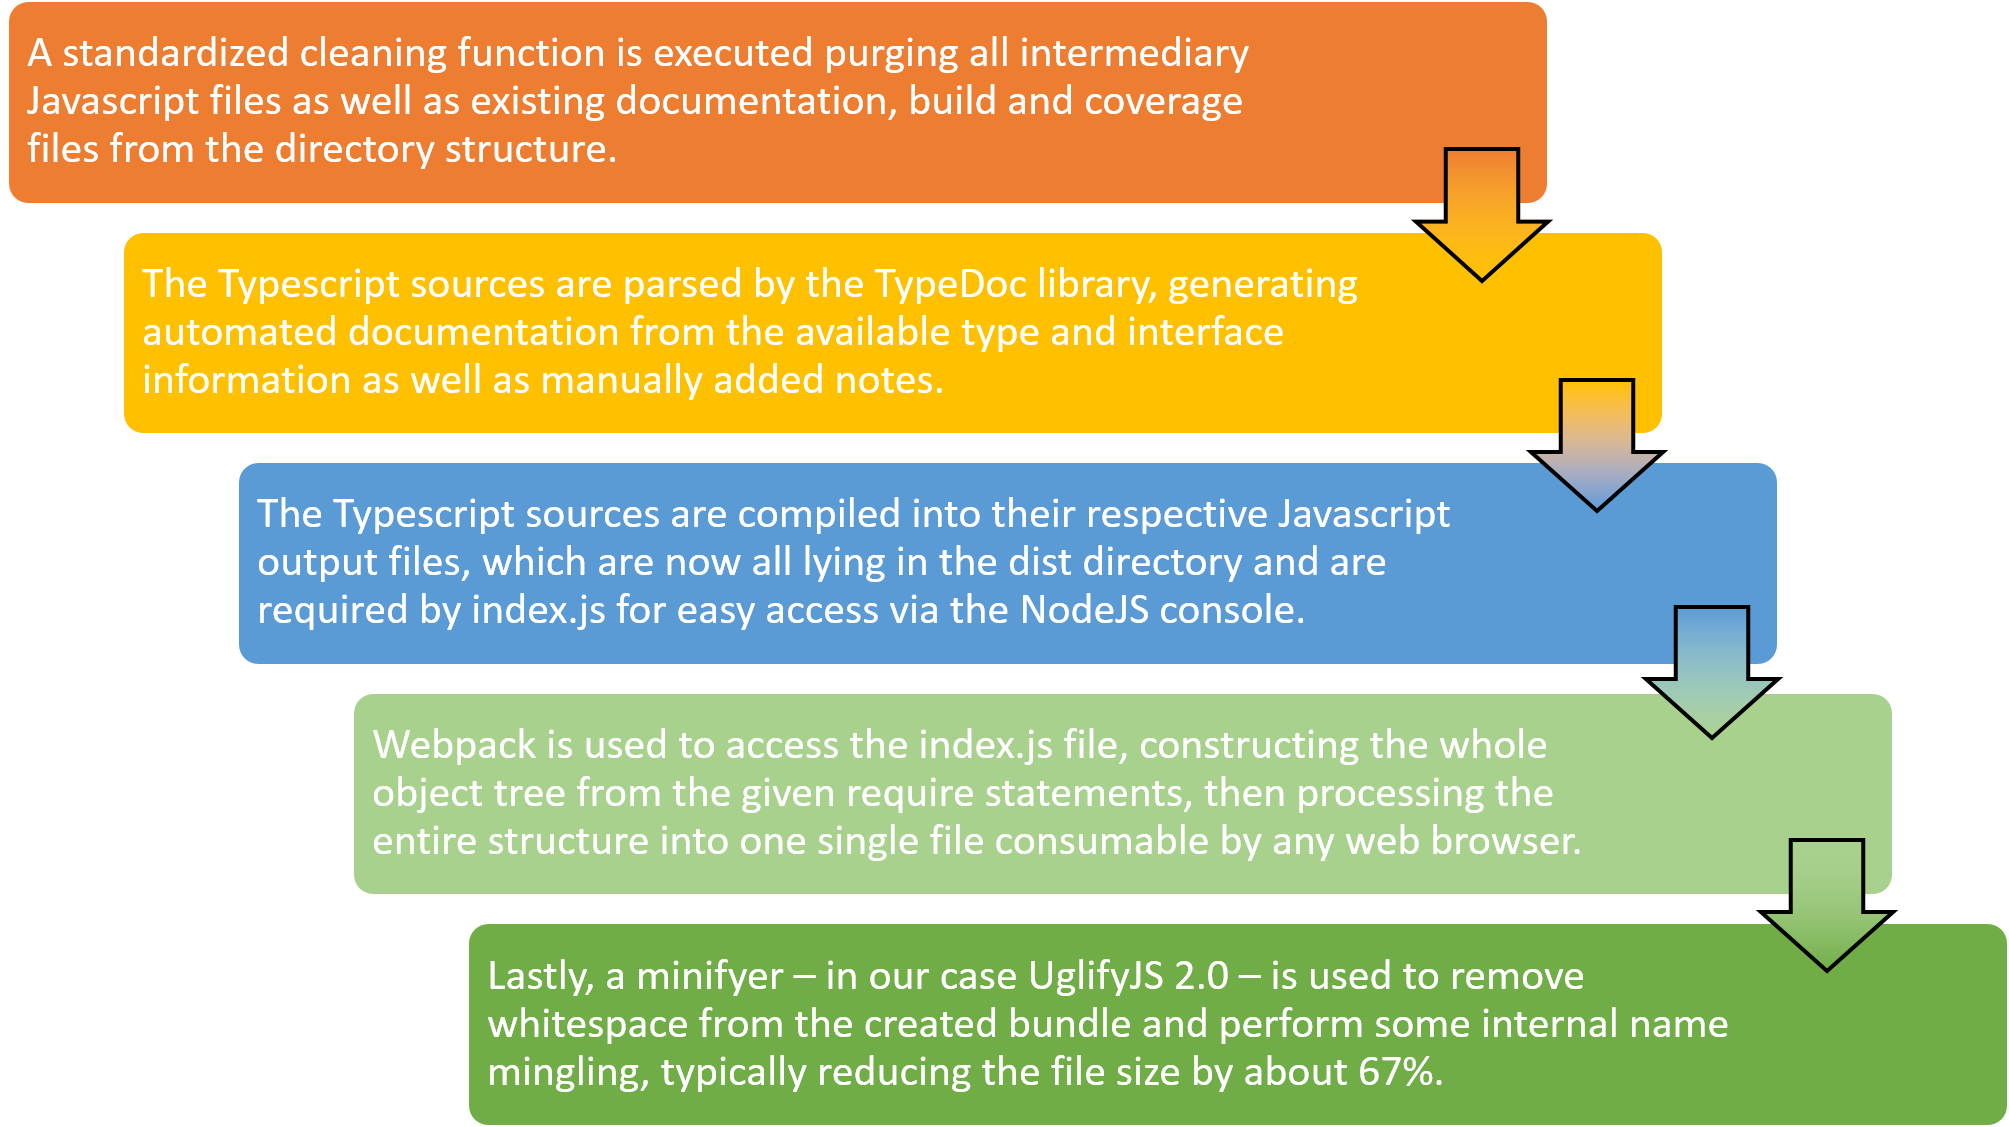
\includegraphics[width=1.1\textwidth]{figures/bundle_process}
	\caption{The GraphiniusJS Bundling process}
\end{figure}


\begin{figure}[ht]
	\label{fig_dependencies}
	\centering
	\hspace*{-0.5cm}
	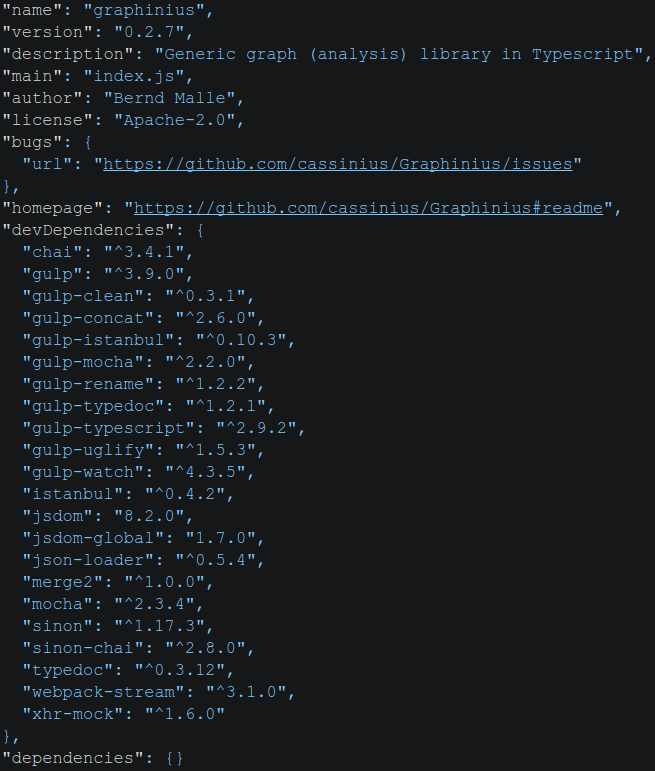
\includegraphics[width=0.8\textwidth]{figures/package_deps}
	\caption{GraphiniusJS development and runtime dependencies}
	\small
	As is clearly visible, I focused on managing all complexity during development time, resulting in zero dependencies for the runtime JS bundle.
\end{figure}



\section{Testing approach}
\label{sect:testing_approach}

	BDD...
	
	\subsection{Unit tests}
	\label{ssect:unittests}
	
	\subsection{Functional tests}
	\label{ssect:func_tests}
	
	\subsection{Mocks used for browser code testing}
	\label{ssect:mocks}

	\subsection{Spies (Sinon)}
	\label{ssect:spies}


\section{Implemented Algorithms}
\label{sect:implemented_algos}

	\subsection{Degree Distribution}
	\label{ssect:deg_dist}

	\subsection{Core Search - Graph Traversal}
	\label{ssect:core_search}
	
		\subsubsection{Breadth first search}
		\label{sssect:search_bfs}
		
		\subsubsection{Depth first search}
		\label{sssect:search_dfs}
		
		\subsubsection{Best (priority) first search}
		\label{sssect:search_pfs}
		
		\subsubsection{Traversal-based algorithms}
		\label{sssect:travseral_algos}
		
		Centralities are 
	
